% 1977 年辽宁卷参考题二：y=Sinx 在 [0,π] 与 x 轴之间的阴影区域（按源卷第 7 页「参考题二附图」布局）
% 源卷图内标注印作「y=Sinπ」，系排印之误，重绘图按 y=Sinx 标注
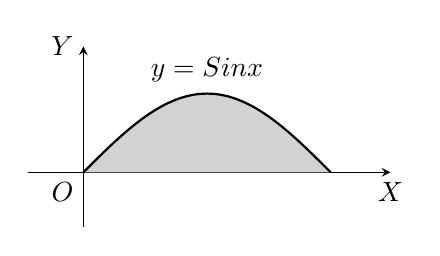
\begin{tikzpicture}[scale=1.0,>=stealth]
  \draw[->] (-0.7,0)--(3.9,0) node[below] {$X$};
  \draw[->] (0,-0.7)--(0,1.6) node[left] {$Y$};
  \node[below left] at (0,0) {$O$};
  \fill[gray!35] (0,0) -- plot[domain=0:3.1416,smooth] (\x,{sin(\x r)}) -- cycle;
  \draw[thick,domain=0:3.1416,smooth] plot (\x,{sin(\x r)});
  \node[draw=none,above] at (1.57,1.02) {$y=\operatorname{Sin}x$};
\end{tikzpicture}
